\chapter{Design Elements}
\label{ch:DesignElements}

This is a normal Paragraph. Note that \textbf{the first paragraph} after a chapter, section, subsection etc. \textbf{has no indentation}. All following paragraphs do have a indentation. Why is that? The function of a paragraph indent is to mark a pause, setting the paragraph apart from what precedes it. If a paragraph is preceded by a title or subhead, the indent is superfluous and can therefore be omitted, as it is here. In \LaTeX{} simply write paragraph text as plain text.

The document uses microtypographical adjustment, such as interletter and interword spacing, gylph expansion, and protrusion. This makes a super nice looking text, aiming to minimize white space and hyphenation.

\section{Structural Elements}

Since we are using a the \tracknshrink{KOMA} class \texttt{scrreprt} (you don’t need to care) we can structure the document in 7 hierarchical layers:

\begin{itemize}
	\setlength\itemsep{-0.75em} % changes the inner item space
	\item \verb|\part{Part title}|
	\item \verb|\chapter{Chapter title}*|
	\item \verb|\section{Section title}*|
	\item \verb|\subsection{Subsection title}*|
	\item \verb|\subsubsection{Subsubsection title}*|
	\item \verb|\paragraph{Paragraph title}|
	\item \verb|\subparagraph{Subparagraph title}|
\end{itemize}


* For this project the items marked with an asterisks are important, I assume. If you need inline headings, as \tracknshrink{APA} and some style guide suggest, you should use the \verb|\paragraph{}| and \verb|\subparagraph{}| commands. As mentioned above, put normal paragraph text in \textbf{no} \LaTeX{} environment.

Note: There is an optional command, in case you’ve got very long chapter, section, etc. headings: \verb|\section[Shorter Title]{Very very long title}|. The shorter title gets displayed in the running header at the top, as well as in the table of contents.

\section{Text Styles}

Use \verb|\textbf{arbitrary words}| to mark words, paragraphs or sections as bold. The output looks like this: \textbf{arbitrary words}. As for italics use \verb|\textit{arbitrary words}|: \textit{arbitrary words}, and small caps \verb|\textsc{arbitrary words}|: \textsc{arbitrary words}. Ultimately, to achieve typewriter style type: \verb|\texttt{arbitrary words}| that will render as: \texttt{arbitrary words}.

\section{Font size}

You might never need to change the font size, since you are using predefined structural elements, that control the font size. Yet, here is a list of \LaTeX{} commands:

\begin{itemize}
	\setlength\itemsep{-0.75em} % changes the inner item space
	\Huge
	\item \verb|\Huge| Text
	\huge
	\item \verb|\huge| Text
	\LARGE
	\item \verb|\LARGE| Text
	\Large
	\item \verb|\Large| Text
	\large
	\item \verb|\large| Text
	\normalsize
	\item \verb|\normalsize| Text
	\small
	\item \verb|\small| Text
	\footnotesize
	\item \verb|\footnotesize| Text
	\scriptsize
	\item \verb|\scriptsize| Text
	\tiny
	\item \verb|\tiny| Text
\end{itemize}

If you change the font size make sure the reset it afterwords with \verb|\normalsize|, otherwise the environment you are working in (e.g. the entire document) takes this size. 

\section{Quote-marks}

This depends on the language defaults. Since this is an English document, we use 66--99 style: “--”. You can either direct input this two glyphs, or you use \verb|``|\textquotesingle{} \textquotesingle{} on your keyboard. \LaTeX{} will interpret this as ``''. Just look at the source code of this file.

\section{Numbers and Mathmodes}

\subsection{Old style figures, FTW!}

Numbers are set to oldstyle figures: 1234567890. If you set numbers in typewriter they are set in typewriter style \texttt{01234567890}. If you would like to suppress oldstyle figures use the \verb|\libertineLF| command right before you type a number; like so: \libertineLF 123, and deactive it afterwards with \verb|\libertineOsF|, so numbers appear in oldstyle again: \libertineOsF 123.

\subsection{Math}

In inline math mode---use \verb|\( Put math here \)|---figures look like so: \(1 + 1 = 2\). Math put on serperate line looks like this:
\begin{alignat*}{2}
	\sigma_1 &= x + y  &\quad \sigma_2 &= \frac{x}{y} \\	
	\sigma_1' &= \frac{\partial x + y}{\partial x} & \sigma_2' 
	&= \frac{\partial \frac{x}{y}}{\partial x}
\end{alignat*}


\section{Lists}

Lists can look like so:

\begin{itemize}
	\setlength\itemsep{-0.75em} % changes the inner item space
	\item one
	\item two
	\item three
\end{itemize}

Check the tex file for syntax.

\section{Abbreviations}

There are three types of \textbf{abbreviation} commands:

\begin{itemize}
	\setlength\itemsep{-0.75em} % changes the inner item space
	\item When you introduce a abv. for the first time use \verb|\acrfull{KEY}|, e.g. \acrfull{CS}
	\item You can also link the long word to the index with \verb|\acrlong{KEY}|, e.g. \acrlong{CS}
	\item But usually you link the short form with \verb|\acrshort{KEY}|, e.g. \acrshort{CS}
\end{itemize}

When you use this commands links and references will be set automatically. If you don’t want to set a reference/link then use the asterisks version of the command: \verb|\acrshort*{KEY}|: \acrshort*{CS}

If you want to add a new abbreviation, go to the \_Abbreviation.tex file. \textbf{Note:} Consider to use the command \verb|\tracknshrink{CAPITAL}| if you abbreviation consists of only capital letters. It’s a common practice in floating text when the letter are tracked and shrinked: USA vs \tracknshrink{USA}. 

\section{Referencing Stuff}

As mentioned above using \verb|acr| code will set references to the list of abbreviation. Most importantly you want to cite literature. 

\subsection{Citing literature}

There are several ways of citing publications:

\begin{itemize}
	\setlength\itemsep{-0.75em} % changes the inner item space
	\item Using \verb|\cite{KEY}|, results in \cite{StaplesBieman1999} and so on 
	\item Using \verb|\parencite{KEY}|, results in \parencite{StaplesBieman1999} and so on 
	\item Using \verb|\textcite{KEY}|, results in \textcite{StaplesBieman1999} and so on 
	\item Using \verb|\citeauthor{KEY}|, results in \citeauthor{StaplesBieman1999} and so on 
	\item Using \verb|\citeyear{KEY}|, results in \citeyear{StaplesBieman1999} and so on 
\end{itemize}

Some citing commands---such as  \verb|\parencite[prefix][suffix]{KEY}|---come with an optional prefix and suffix notation. The prefix usually makes sense for the word: \textit{see} to compare something similar or to put the word \textit{cf.} to contrast something. Suffix is handy for page numbers. A \textit{p.} gets inserted, automatically. Usually you use this with \verb|\parencite|:

\begin{itemize}
	\setlength\itemsep{-0.75em} % changes the inner item space
	\item Using \verb|\parencite[see][96]{KEY}|, results in \parencite[see][96]{StaplesBieman1999} and so on
	\item Using \verb|\parencite[cf.][64]{KEY}|, results in \parencite[cf.][64]{StaplesBieman1999} and so on 
\end{itemize}

If you use only one bracket the suffix variant gets used: \textcite[97]{StaplesBieman1999} discuss in their publication \textellipsis

\subsection{Referencing Section, Figures, Tables, etc.}

You can reference to everything which has a label or a caption. If you set a label or a caption, it’s a good practice to use prefixes: Figures: fig: -- Tables: tab: -- Source code: lst: -- Chapters: ch: -- Sections: sec: -- Subsections: ssec: and so on.

There are 3 keywords to consider:

\begin{itemize}
	\setlength\itemsep{-0.75em} % changes the inner item space
	\item \verb|\autoref{ch:DesignElements}| looks like: \autoref{ch:DesignElements} --- Depending on what you reference the name will adapt (Figure, Table, Code, Section, etc.)
	\item \verb|\nameref{ch:DesignElements}| looks like: \nameref{ch:DesignElements} --- This is giving you the caption of the element or the title
	\item \verb|\pageref{ch:DesignElements}| looks like: \pageref{ch:DesignElements} --- This is giving you the page of the element
\end{itemize}

Use the \verb|\href{URL}{LINK TEXT}| command for external links. Yet, it is better to use \verb|\url{URL}|. Since in printed form the link wont be obfuscated, and the latter one handles line breaks while href does not.

\section{Pictures}

Please please please use vector graphics in pdf format, if available. For sure take jpg if you want to show photos.

\subsection{Using a simple picture}

\begin{figure}[H]
	\centering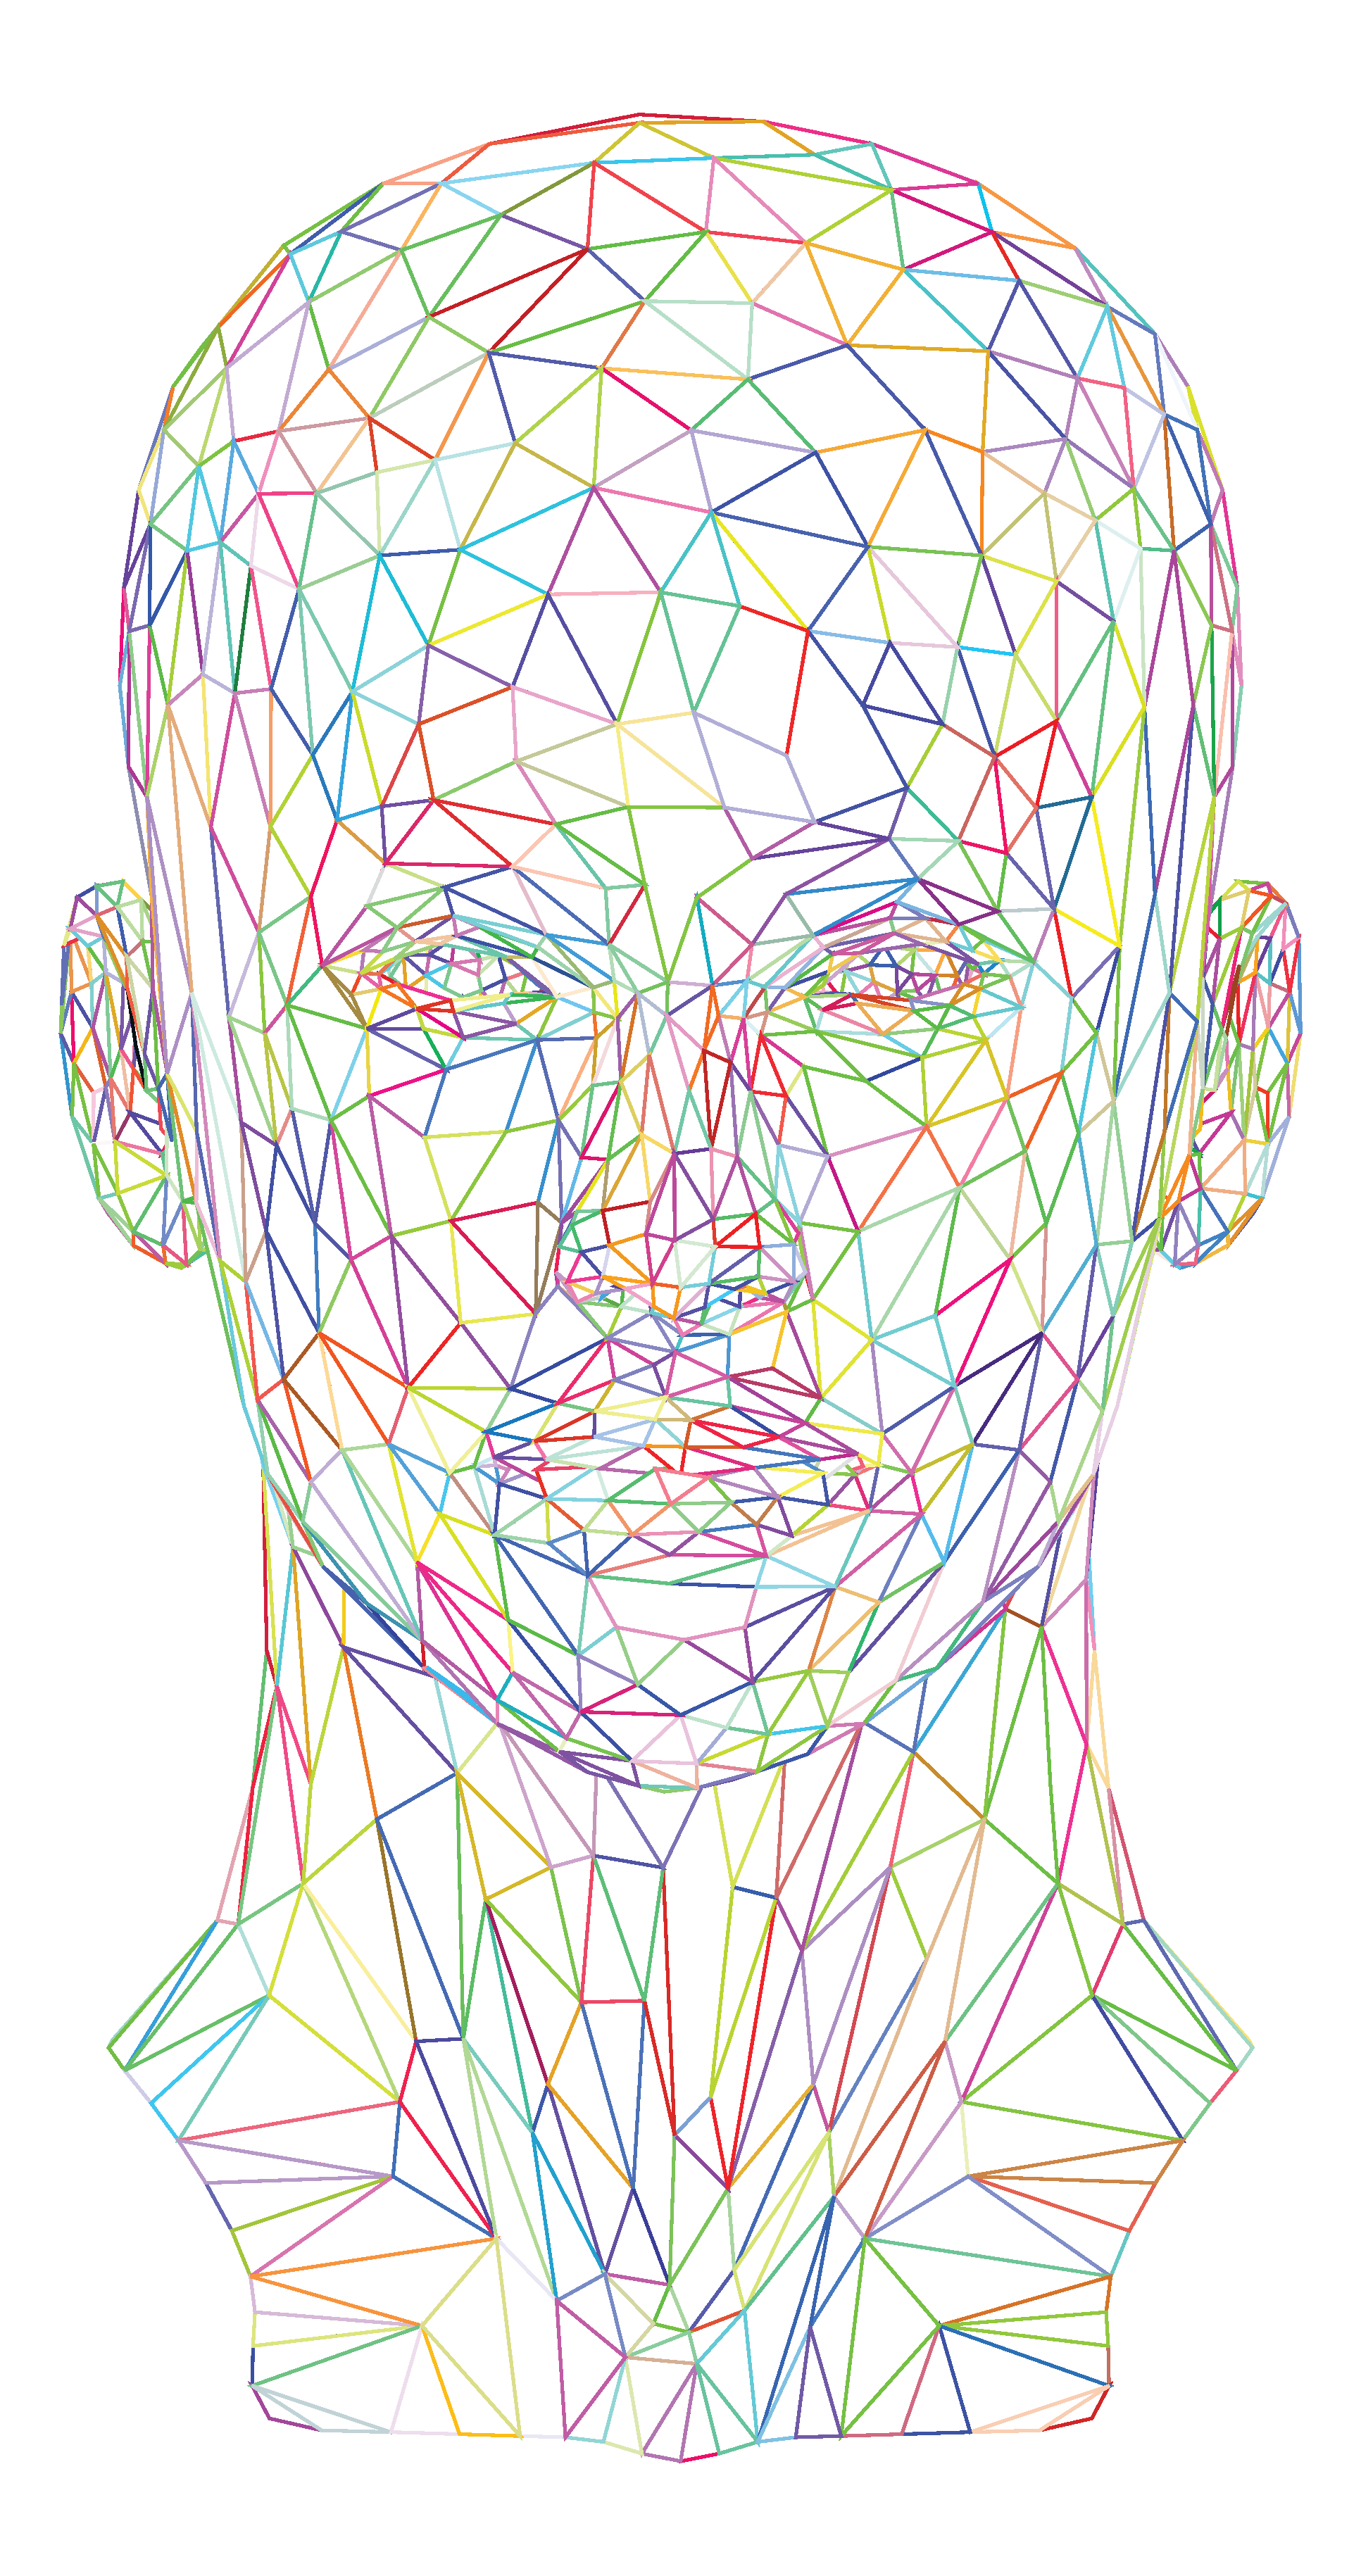
\includegraphics[width=3cm]{wireframehead.pdf}
	\caption[Optional shorter List of Figures Caption]{This caption can be really long since with use the optional brackets for the smaller caption that will be displayed in the list of figures.}
	\label{fig:WireframeHead}
\end{figure}


\subsection{Using a picture overlays}

See the \texttt{.tex} file for instructions. When you plan to use overlays you usually use a grid to set exact coordinate points where you want your anchors to be. When you’re done, you simplay comment out the grid.


\begin{figure}[H]
	\libertineLF
	\centering \begin{tikzpicture}
	\node[anchor=south west,inner sep=0] (image) at (0,0,0) {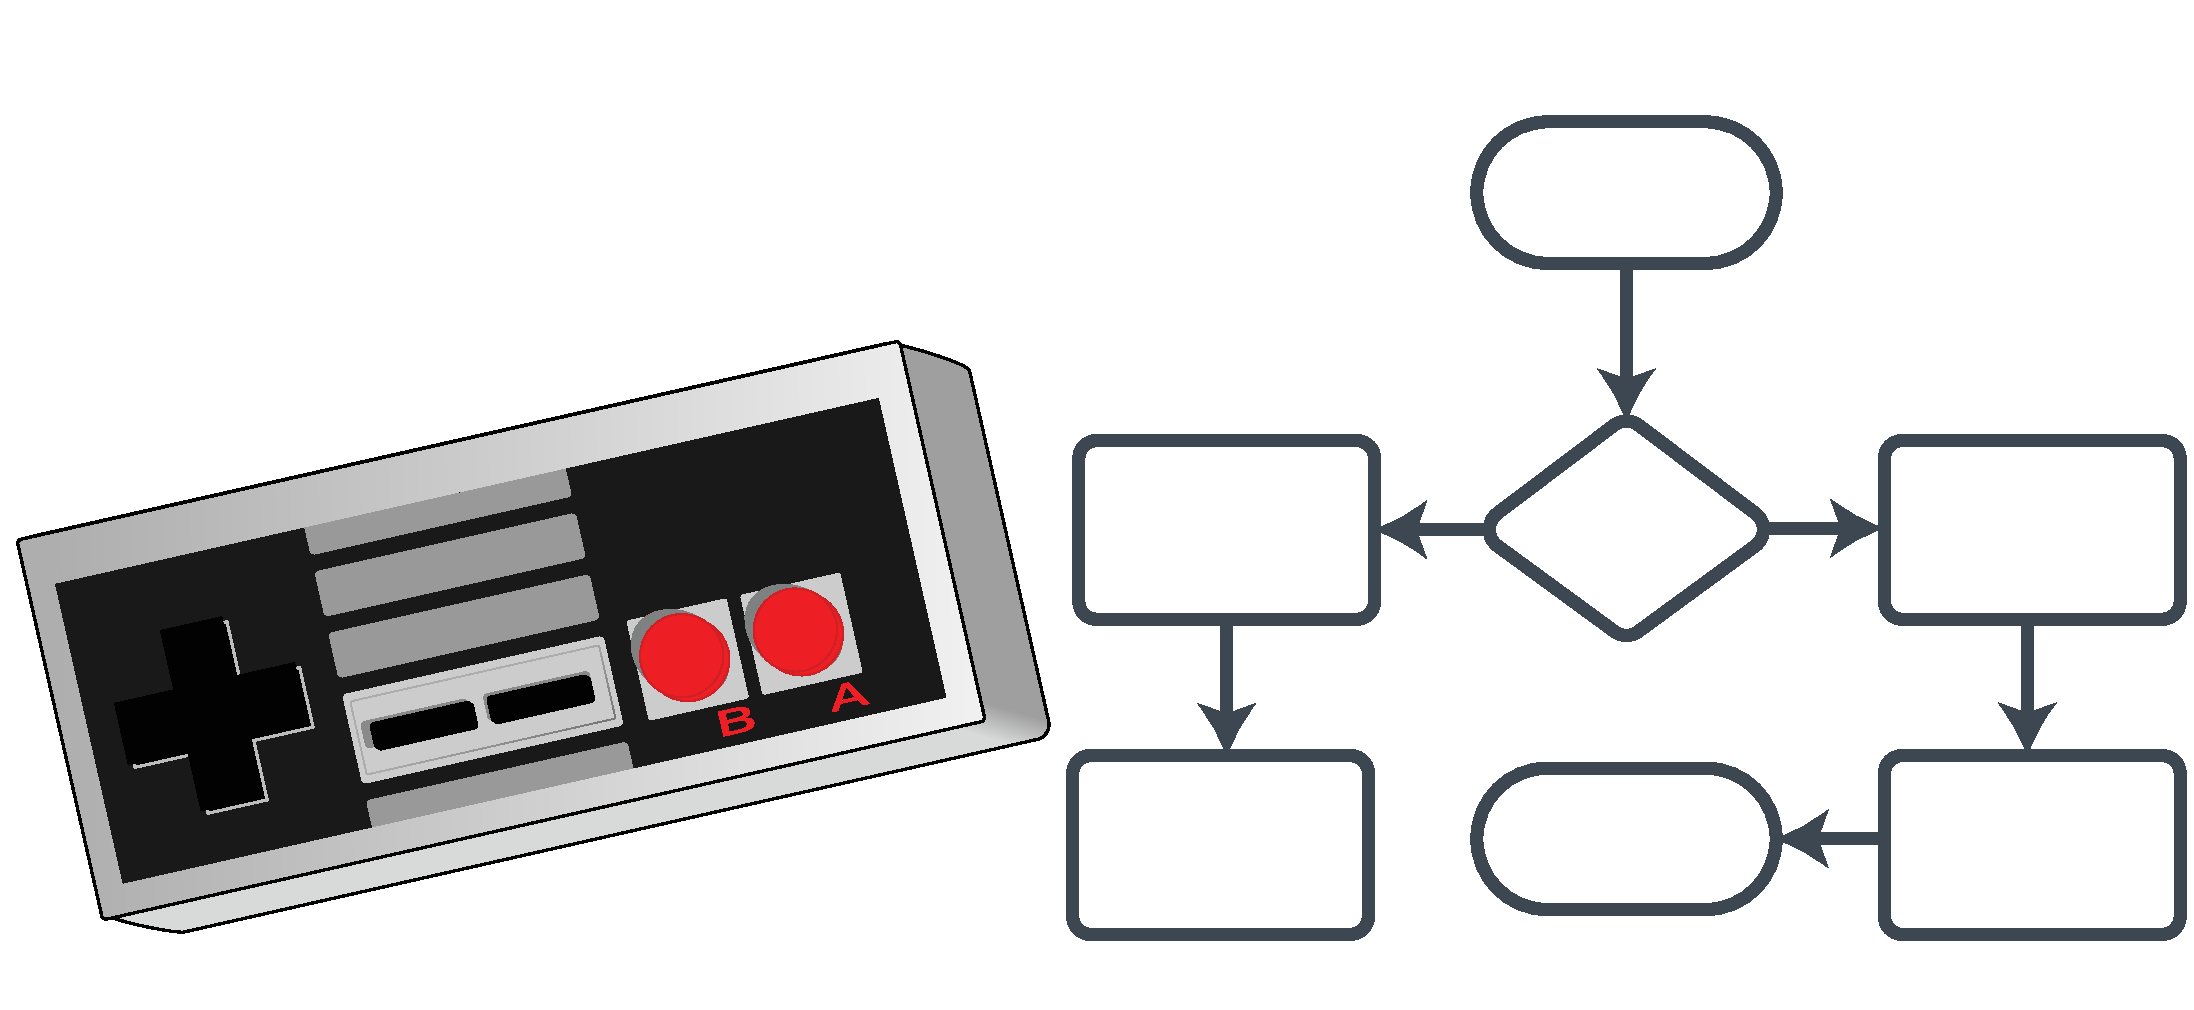
\includegraphics[width=8cm]{compare.pdf}};
	\begin{scope}[x={(image.south east)},y={(image.north west)}]
	% next four lines will help you to locate the point needed by forming a grid. comment these four lines in the final picture.↓
		\draw[help lines,xstep=.1,ystep=.1] (0,0) grid (1,1);
		\draw[help lines,xstep=.05,ystep=.05] (0,0) grid (1,1);
		\foreach \x in {0,1,...,9} { \node [anchor=north] at (\x/10,0) {0.\x}; }
		\foreach \y in {0,1,...,9} { \node [anchor=east] at (0,\y/10) {0.\y};}
	% upto here↑
	
	\draw (0.25,1) node {(A)};
	\draw (0.75,1) node {(B)};
	
	\draw[dashed,-latex] (0.5,0.488) -- +(-2.8cm,1cm)node[anchor=east] {(1)};
	\draw[dashed,-latex] (0.75,0.65) -- +(1.5cm,1cm)node[anchor=west] {(2)};
	\draw[dashed,-latex] (0.9,0.3) -- +(0.75cm,-0.5cm)node[anchor=west] {(3)};
	
	\draw[-latex] (0.003,0.003) -- +(-0.5cm,0cm)node[anchor=east] {{\tiny Arrows with straight lines}};
	\draw[-latex] (0.997,0.003) -- +(+0.5cm,0cm)node[anchor=west] {{\footnotesize Smaller text}};
	\draw[-latex] (0.997,0.501) -- +(+0.5cm,0cm)node[anchor=west] {0,1,2};
	\draw[-latex] (0.003,0.501) -- +(-0.5cm,0cm)node[anchor=east] {Text};
	\draw[-latex] (0.503,0.997) -- +(+0.5cm,0.5cm)node[anchor=west] {Some random text};
	
	\draw [fill=black] (0.003,0.003) circle (.3ex);
	\draw [fill=black] (0.997,0.003) circle (.3ex);
	\draw [fill=black] (0.997,0.501) circle (.3ex);
	\draw [fill=black] (0.003,0.501) circle (.3ex);
	\draw [fill=black] (0.503,0.997) circle (.3ex);
	
	\end{scope}
	\end{tikzpicture}
	\caption[Demonstrating the grid view]{Demonstrating the grid view}
	\label{fig:gridView}
	\libertineOsF
\end{figure}

When you are done with arranging your shit, you simply comment out the grid:

\begin{figure}[H]
	\libertineLF
	\centering \begin{tikzpicture}
	\node[anchor=south west,inner sep=0] (image) at (0,0,0) {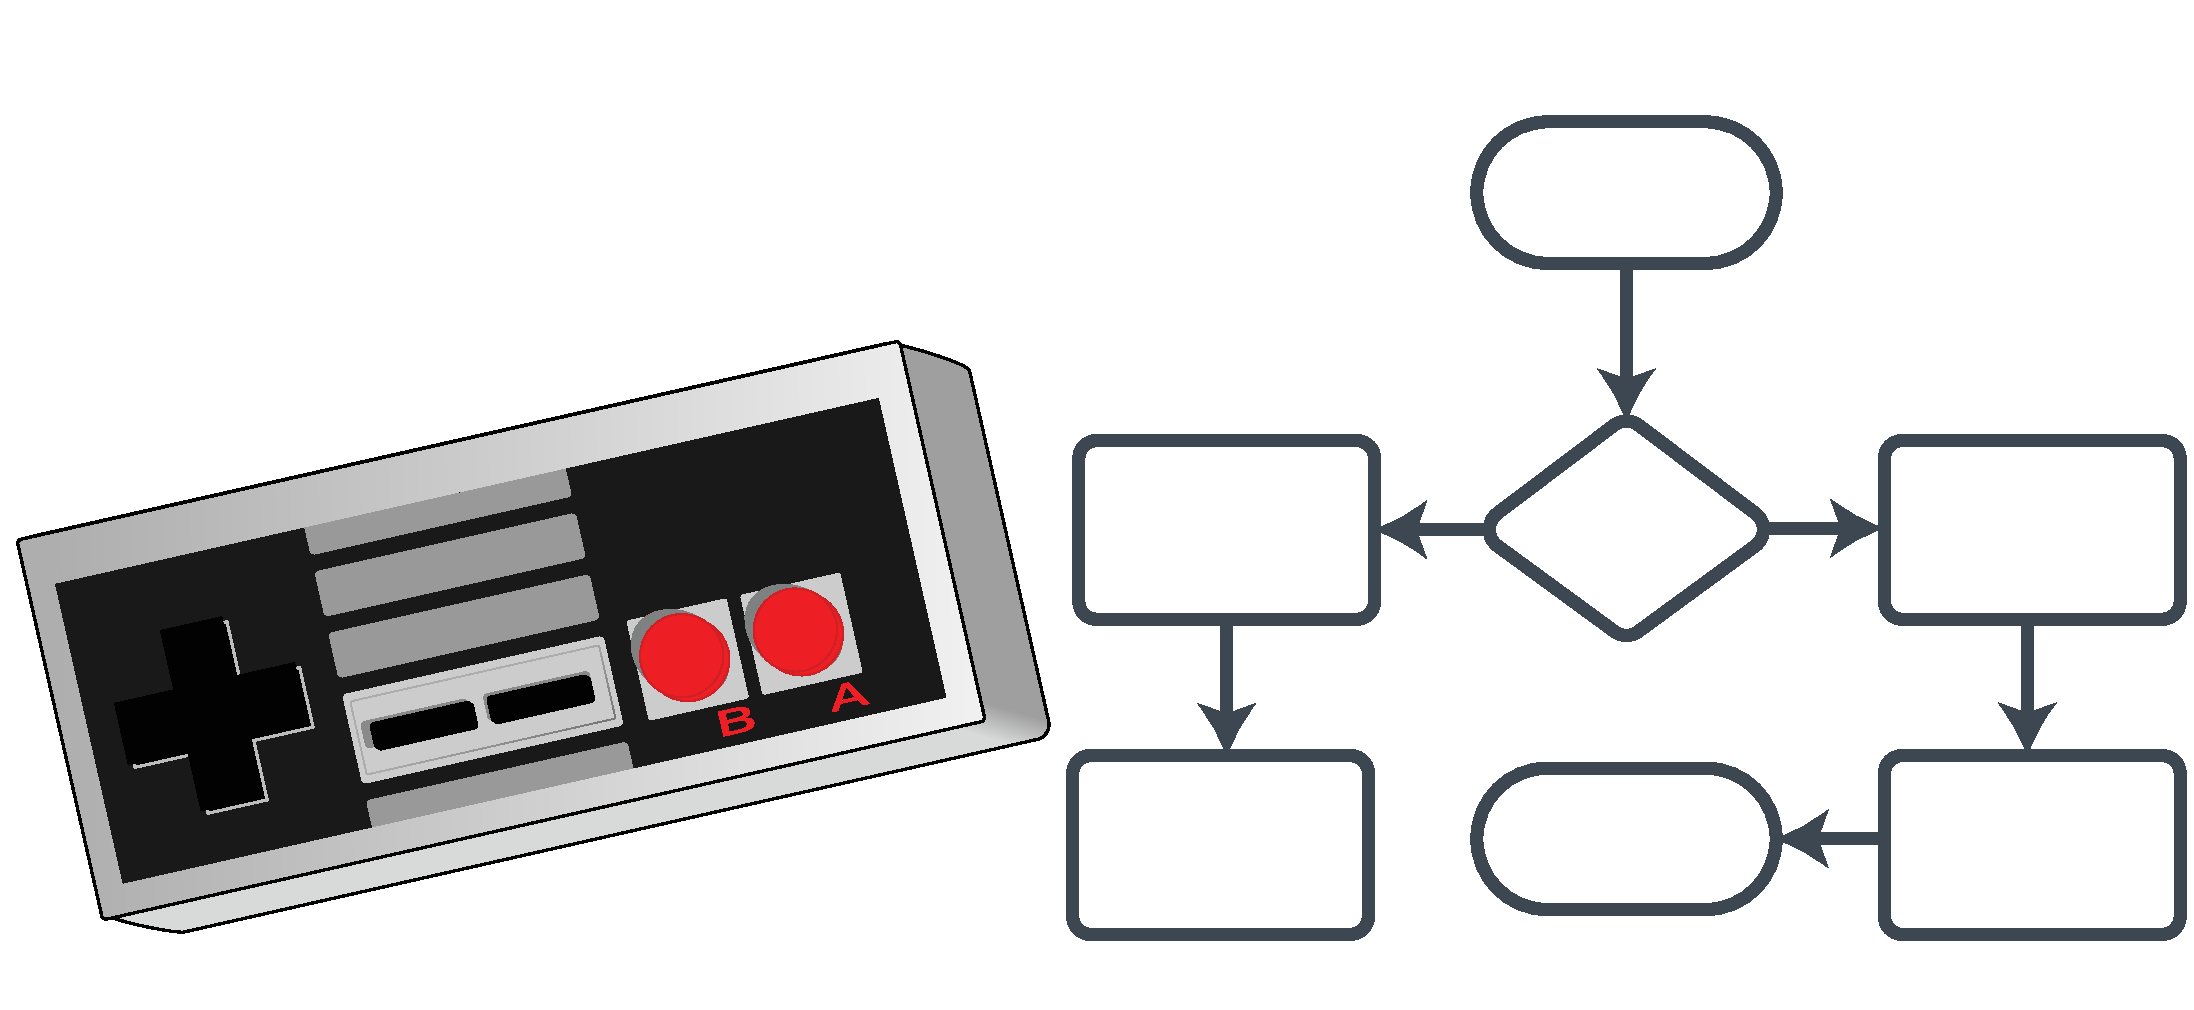
\includegraphics[width=8cm]{compare.pdf}};
	\begin{scope}[x={(image.south east)},y={(image.north west)}]
%	% next four lines will help you to locate the point needed by forming a grid. comment these four lines in the final picture.↓
%	\draw[help lines,xstep=.1,ystep=.1] (0,0) grid (1,1);
%	\draw[help lines,xstep=.05,ystep=.05] (0,0) grid (1,1);
%	\foreach \x in {0,1,...,9} { \node [anchor=north] at (\x/10,0) {0.\x}; }
%	\foreach \y in {0,1,...,9} { \node [anchor=east] at (0,\y/10) {0.\y};}
%	% upto here↑
	
	\draw (0.25,1) node {(A)};
	\draw (0.75,1) node {(B)};
	
	\draw[dashed,-latex] (0.5,0.488) -- +(-2.8cm,1cm)node[anchor=east] {(1)};
	\draw[dashed,-latex] (0.75,0.65) -- +(1.5cm,1cm)node[anchor=west] {(2)};
	\draw[dashed,-latex] (0.9,0.3) -- +(0.75cm,-0.5cm)node[anchor=west] {(3)};
	
	\draw[-latex] (0.003,0.003) -- +(-0.5cm,0cm)node[anchor=east] {{\tiny Arrows with straight lines}};
	\draw[-latex] (0.997,0.003) -- +(+0.5cm,0cm)node[anchor=west] {{\footnotesize Smaller text}};
	\draw[-latex] (0.997,0.501) -- +(+0.5cm,0cm)node[anchor=west] {0,1,2};
	\draw[-latex] (0.003,0.501) -- +(-0.5cm,0cm)node[anchor=east] {Text};
	\draw[-latex] (0.503,0.997) -- +(+0.5cm,0.5cm)node[anchor=west] {Some random text};
	
	\draw [fill=black] (0.003,0.003) circle (.3ex);
	\draw [fill=black] (0.997,0.003) circle (.3ex);
	\draw [fill=black] (0.997,0.501) circle (.3ex);
	\draw [fill=black] (0.003,0.501) circle (.3ex);
	\draw [fill=black] (0.503,0.997) circle (.3ex);
	
	\end{scope}
	\end{tikzpicture}
	\caption[Demonstrating the result]{Demonstrating the result}
	\label{fig:nongridView}
	\libertineOsF
\end{figure}

\section{Change Languages}

It is important to tell \LaTeX{} if a different language is used, because of language specific hyphenation, ligature, and characters (change from “...” to „...“, etc.). You can find more information here: \url{https://en.wikibooks.org/wiki/LaTeX/Internationalization#Babel}.

E.g. to change to German language use: \verb|\begin{otherlanguage}{ngerman}|, to tell Babel to change to German, like the following paragraph:

\begin{otherlanguage}{ngerman}
Dr. Heinrich Faust ist ein angesehener Wissenschaftler und Akademiker, der trotz seiner wissenschaftlichen Studien und einer guten Bildung seinen Wissensdurst nicht stillen kann. Eines Nachts sitzt er in seinem Studierzimmer und grübelt über den Sinn des Lebens nach, findet jedoch keine Antworten.
\end{otherlanguage}

\section{Tables}

\begin{table}[H]\centering
	\libertineLF
	\begin{tabular}{l*{3}{c}}
		\toprule
		&     Base   &   Robust   &  Cluster   \\
		&\multicolumn{1}{c}{(1)}   &\multicolumn{1}{c}{(2)}   &\multicolumn{1}{c}{(3)}   \\
		\midrule
		Size            &-0.000645   &-0.000645   &-0.000645   \\
		&  (-0.83)   &  (-0.83)   &  (-0.39)   \\
		\midrule
		Observations    &     5035   &     5035   &     5035   \\
		\bottomrule
		\multicolumn{4}{l}{\footnotesize \textit{t} statistics in parentheses}\\
		\multicolumn{4}{l}{\footnotesize *\( p<0.10, ** p<0.05, *** p<0.01\)}\\
	\end{tabular}
	\caption[Short Heading]{Hey there}
	\label{tab:Observations}
	\libertineOsF
\end{table}

\begin{table}[H]\centering
	\libertineLF
\begin{tabular}{lrr} 
	\toprule
	\multicolumn{2}{c}{Studium}\\ \cmidrule{1-2}
	Fach & Dauer & Einkommen (\euro{})\\ 
	\midrule 
	Info & 2 & 12,75 \\ \addlinespace
	MST & 6 & 8,20 \\ \addlinespace
	VWL & 14 & 10,00\\ 
	\bottomrule
\end{tabular}
	\caption[Another table]{Yet another table. It’s number 2.}
	\label{tab:Money}
	\libertineOsF
\end{table}

\begin{table}[H]\centering
	\libertineLF
\begin{tabular}{llll} \toprule
	Organismen Name & Substratfreie Kontrolle  & \multicolumn{2}{c}{Probenansatz} \\\cmidrule(rl){3-4}
	& Farbe & Farbe & Bewertung \\\midrule
	Alpha1 & farblos &  dunkel braun & +++ \\
	MaT2 & farblos & farblos & - \\\bottomrule
\end{tabular}
	\caption[Even more tables]{Yet another table. It’s number 3.}
	\label{tab:Organics}
	\libertineOsF
\end{table}

\begin{table}[H]\centering
	\libertineLF
\begin{tabular}{lccc}\toprule
	\textbf{Stoff}	&\textbf{Dichte} &\textbf{Dichte} &\textbf{Chemische Bezeichnung}	\\
	& \(kg/m^{3}\)	& \(g/cm^3\) 	& \\\midrule
	Holz		& 400...800	& 0,400...0,800	&- \\
	Plexiglas 	& 1190	& 1,19	& - 	\\
	Aluminium	& 2710	& 2,71	& Al	\\
	Titan		& 4500	& 4,5	& Ti	\\
	Gusseisen	& 7250	& 7,25	& - \\
	Stahl legiert& 7900	& 7,9	& - \\
	Messing		& 8.100...8.700	& 8,100...8,700	& Cu-Zn-Legierung\\
	Konstantan	& 8800	& 8,8	& Cu55Ni45-Legierung\\
	Nickel		& 8910	& 8,91  & Ni \\
	Kupfer		& 8.920...8.960	& 8,920...8,960	& Cu\\
	Gold		& 19302	& 19,302& Au	\\\bottomrule
\end{tabular}
	\caption[OMG! Even more tables]{Yet another table. It’s number 4.}
	\label{tab:Chemistry}
	\libertineOsF
\end{table}

Notice the alignment of following table:
\begin{table}[H]\centering
	\libertineLF
\begin{tabular}{SSSSSSSS} \toprule
	{$m$} & {$\Re\{\underline{\mathfrak{X}}(m)\}$} & {$-\Im\{\underline{\mathfrak{X}}(m)\}$} & {$\mathfrak{X}(m)$} & {$\frac{\mathfrak{X}(m)}{23}$} & {$A_m$} & {$\varphi(m)\ /\ ^{\circ}$} & {$\varphi_m\ /\ ^{\circ}$} \\ \midrule
	1  & 16.128 & +8.872 & 16.128 & 1.402 & 1.373 & -146.6 & -137.6 \\
	2  & 3.442  & -2.509 & 3.442  & 0.299 & 0.343 & 133.2  & 152.4  \\
	3  & 1.826  & -0.363 & 1.826  & 0.159 & 0.119 & 168.5  & -161.1 \\
	4  & 0.993  & -0.429 & 0.993  & 0.086 & 0.08  & 25.6   & 90     \\ \midrule
	5  & 1.29   & +0.099 & 1.29   & 0.112 & 0.097 & -175.6 & -114.7 \\
	6  & 0.483  & -0.183 & 0.483  & 0.042 & 0.063 & 22.3   & 122.5  \\
	7  & 0.766  & -0.475 & 0.766  & 0.067 & 0.039 & 141.6  & -122   \\
	8  & 0.624  & +0.365 & 0.624  & 0.054 & 0.04  & -35.7  & 90     \\ \midrule
	9  & 0.641  & -0.466 & 0.641  & 0.056 & 0.045 & 133.3  & -106.3 \\
	10 & 0.45   & +0.421 & 0.45   & 0.039 & 0.034 & -69.4  & 110.9  \\
	11 & 0.598  & -0.597 & 0.598  & 0.052 & 0.025 & 92.3   & -109.3 \\ \bottomrule
\end{tabular}
	\caption[Table with nice alignment]{Table with nice alignment}
	\label{tab:Alignment}
	\libertineOsF
\end{table}

\newpage

\section{Code Listings}

\lstset{language=Java}
\begin{lstlisting}[
label={lst:BubbleSort},
xleftmargin=12em, % this needs to be manually adjusted to center the frame
xrightmargin=-12em, % this needs to be manually adjusted to center the frame
caption={[Bubblesort in Java]Bubblesort in Java}]
public static int[] bubblesort(int[] numbers) {
	boolean swapped = true;
	for(int i = numbers.length - 1; i > 0 && swapped; i--) {
		swapped = false;
		for (int j = 0; j < i; j++) {
			if (numbers[j] > numbers[j+1]) {
			int temp = numbers[j];
			numbers[j] = numbers[j+1];
			numbers[j+1] = temp;
			swapped = true;
			}
		}
	}
	return numbers;
}
\end{lstlisting}

\section{Using TODO Notes}

You can add todo notes easily with \todo{Your text} \verb|\todo{Your text}|. You see the result on the right margin. This project uses additionally some predefined todo labels:

\begin{itemize}
	\setlength\itemsep{-0.75em} % changes the inner item space
	\item use \verb|\unsure{Are you sure?}| \unsure{Are you sure?} to express uncertainty.
	\item use \verb|\citethis{Citation missing!}| \citethis{Citation missing!} if you miss a citation.
	\item use \verb|\info{Hint: yada yada.}| \info{Hint: yada yada.} to provide some information.
	\item use \verb|\wording{Too colloquial!}| \wording{Too colloquial!} if wording is too complex, colloquial, etc.
\end{itemize}

Use the option \verb|\todo,unsure,citethis,info,wording[inline]{Your inline text}| to create inline todo:
\wording[inline]{The following sections sounds shit}

Inline todos tend to throw overfull hboxes. Yet, you can ignore that.



\newpage
\listoftodos[All TODOs]

